\subsection{Risikoanalyse}

Jedes Projekt birgt Risiken. Diese Risiken können sich auf die Projektdauer, die Kosten oder die Qualität auswirken. Um diese Risiken zu minimieren, wird eine Risikoanalyse erstellt. Zuerst werden die Risiken identifiziert und wie diese Risiken eintreten können. Anschließend werden Maßnahmen erarbeitet, die gegen diese Risiken getroffen werden sollen. Die Wahrscheinlichkeit, dass diese Risiken eintreten, wird ebenfalls ermittelt. Unabhängig davon, wie detailliert eine Risikoanalyse ausgearbeitet wird, ist es dennoch immer wichtig mit unidentifizierten Risiken zu rechnen. Auch während des Projektverlaufs können neue Risiken auftreten und müssen dann ebenfalls berücksichtigt und laufend zur Risikoanalyse hinzugefügt werden \citev{risikomanagement}. In der Tabelle \ref{tab:risikoanalyse} werden Risiken, die das Projektteam identifiziert hat aufgelistet.

Kosten des endgültigen Produktes haben für die Diplomarbeit keine Relevanz. Trotzdem werden die Kosten und die damit verbundenen Risiken miteinbezogen. Falls das Projekt weiter verfolgt wird, werden Kosten relevanter und haben dadurch auch ein höheres Risiko.

% TODO fix alignment
\begin{table}[H]
  \centering
  \small
  \begin{tabular}{c|p{0.15\textwidth}|p{0.3\textwidth}|p{0.3\textwidth}|c}
    \multicolumn{5}{c}{\textbf{Risikoanalyse}}                                                                                                                                                                                                                                                                                   \\
    \toprule
    \textbf{ID} & \textbf{Risiko}                                    & \textbf{Mögliche Risikoursachen}                                                                                       & \textbf{Maßnahmen}                                                                                                 & \textbf{\%} \\
    \midrule
    R1          & Projekt wird nicht rechtzeitig fertig              & Produktmanagement- bzw. Planungsfehler, interne und externe Kommunikation funktioniert nicht, Projektumfang nicht klar & Pufferzeiten einplanen, Projekt detailliert planen                                                                 & 10\%        \\ \ghline
    R2          & Umsetzung zu kostspielig                           & Varianten nicht ausreichend analysiert, Fehlplanung, Fehlkonstruktion                                                  & Genaue Kostenrechnung durchführen, Businessplan erstellen, innovativere Varianten konzeptionieren                  & 50\%        \\ \ghline
    R3          & \enquote{Projektmitarbeiter} erledigt Arbeit nicht & \enquote{Projektmitarbeiter} ist krank oder anderweitig beschäftigt                                                    & \enquote{Projektmitarbeiter} übernimmt keine kritischen Aufgaben, geringeres Arbeitspensum, Pufferzeiten einplanen & 45\%        \\
    \bottomrule
  \end{tabular}
  \caption{Risikoanalyse}
  \label{tab:risikoanalyse}
\end{table}

\begin{figure}[H]
  \centering
  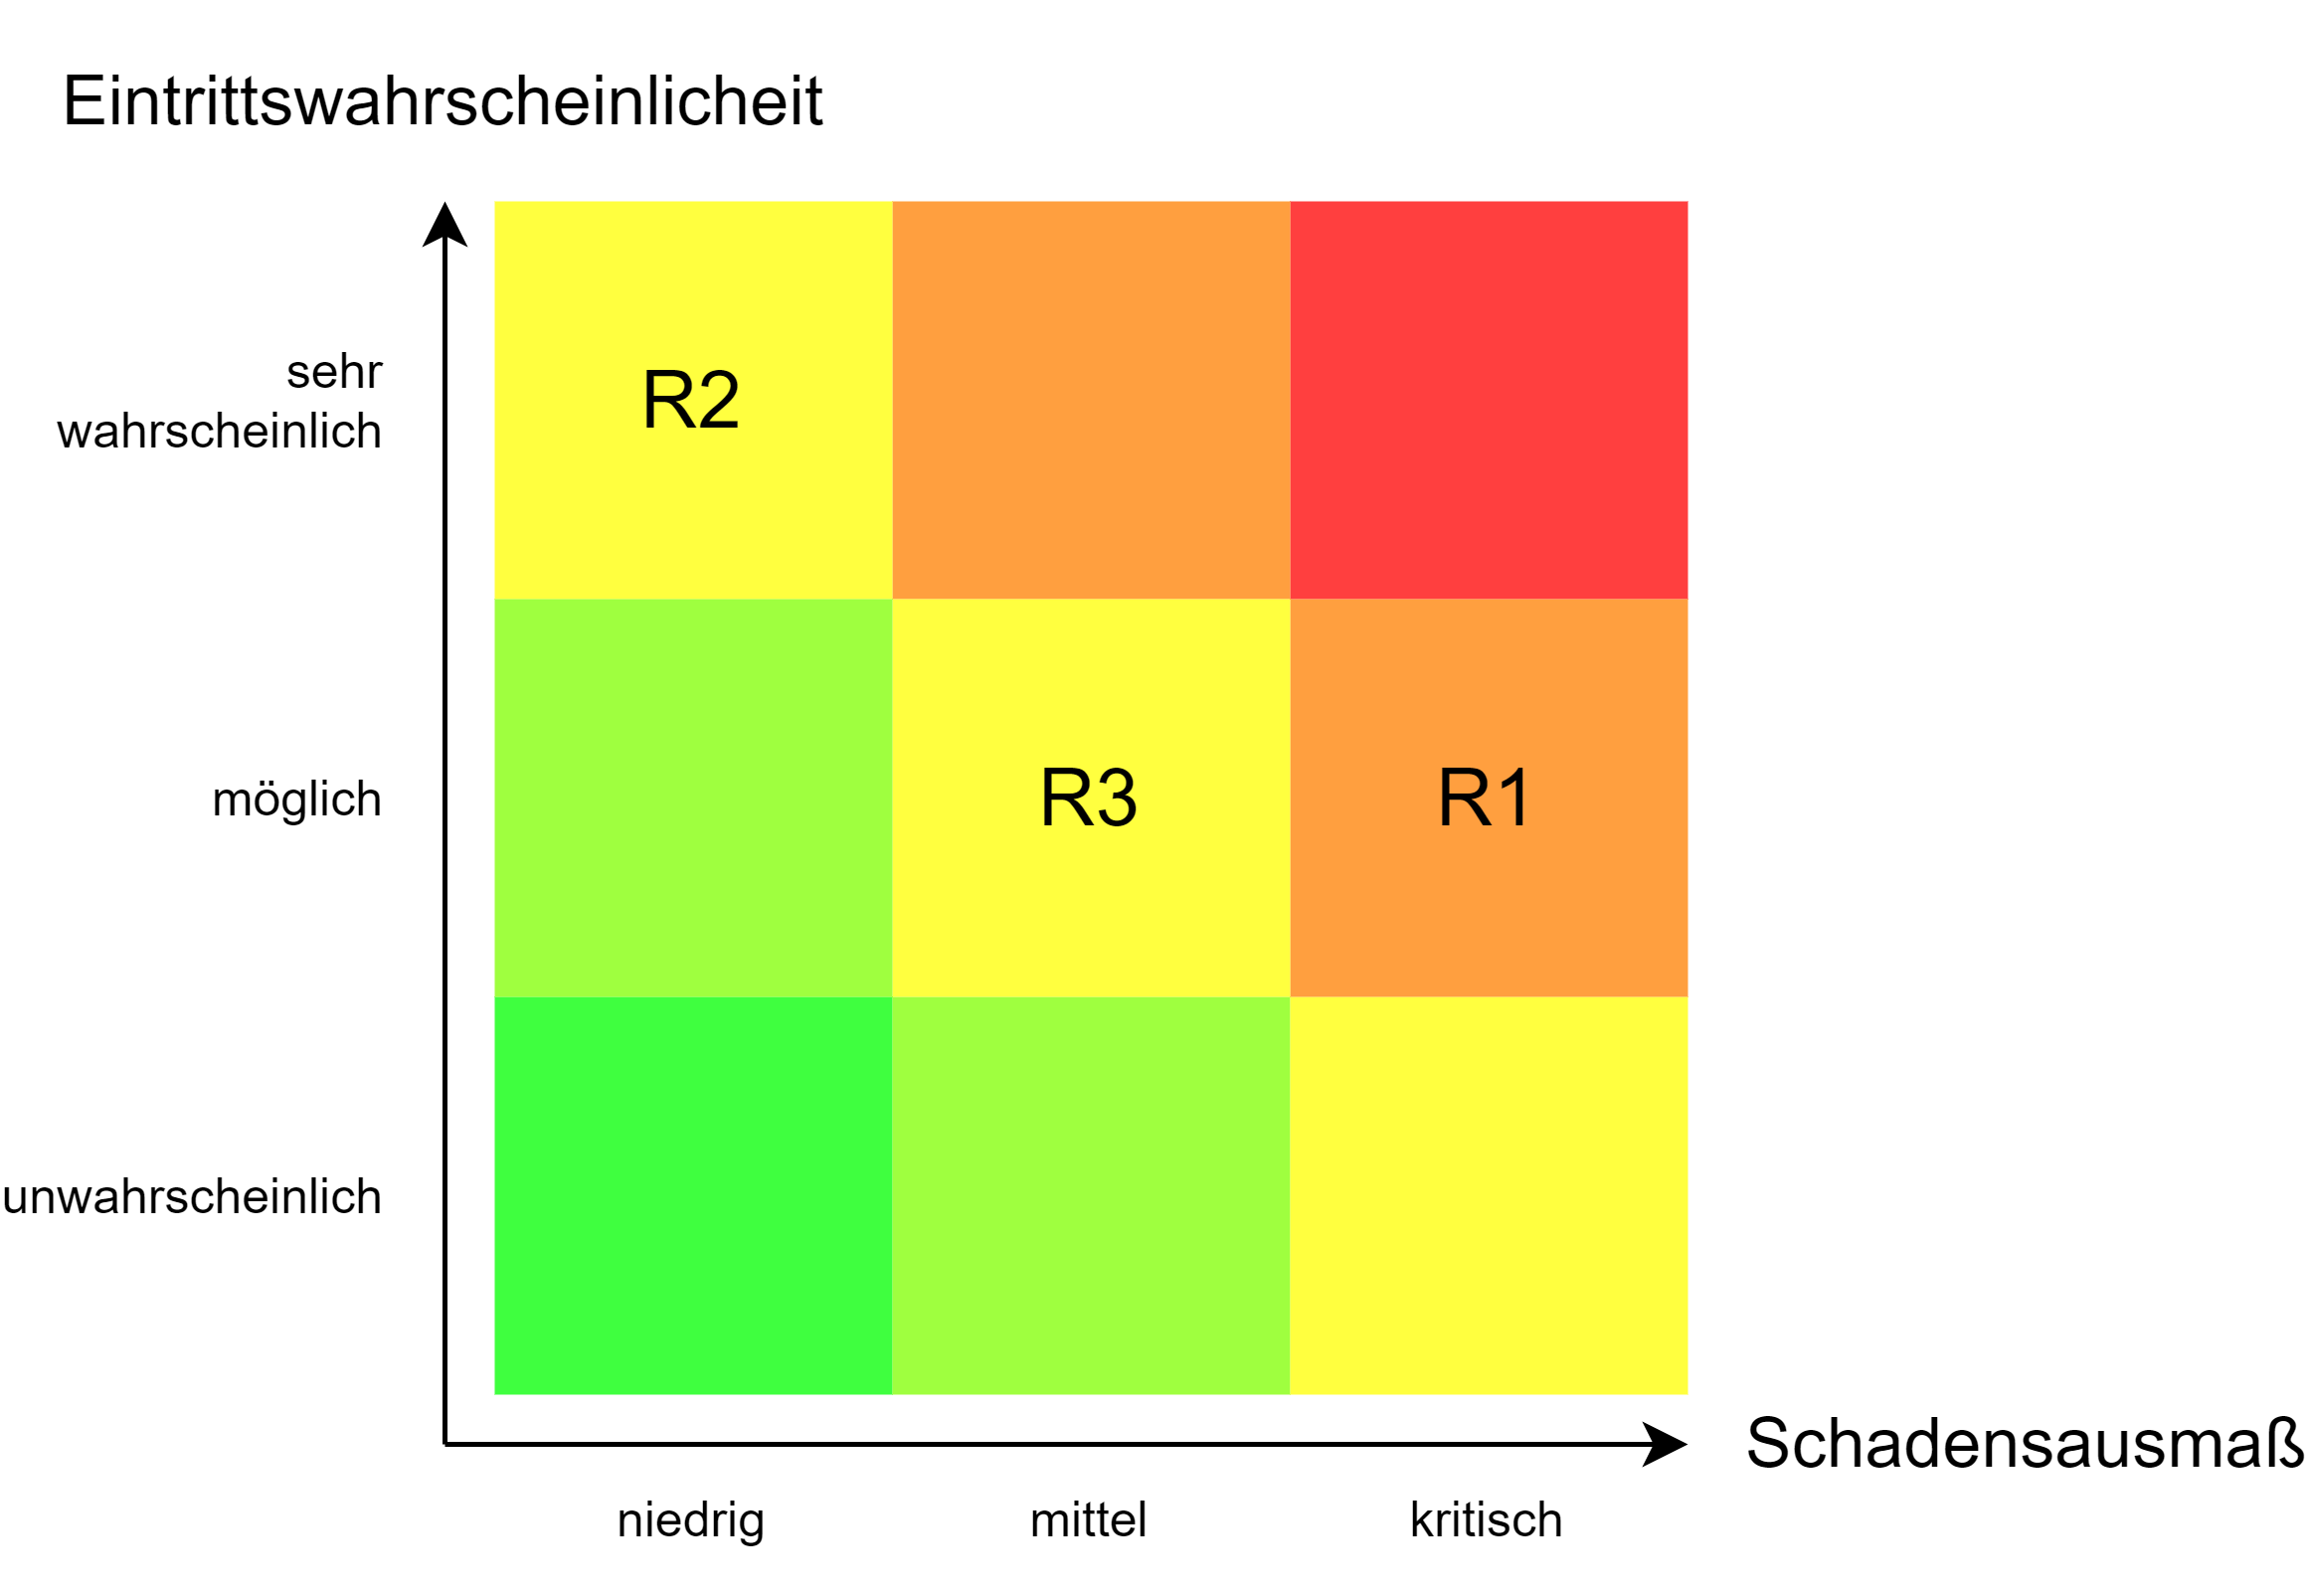
\includegraphics[width=0.75\textwidth]{images/risikoanalyse.png}
  \caption{Risikoanalyse Matrix}
  \label{fig:risikoanalyse_matrix}
\end{figure}